\documentclass{article}

\usepackage{array}
\usepackage{graphicx}

\begin{document}

\title{Week 9, Session 2 Problems}
\author{GSI: Caleb Eades}
\date{10/18}
\maketitle

\section{Capacitors}

\subsection{Cylindrical Capacitor}

Calculate the capacitance of a pair of cylinders of radii $a$ and $b$ and length $l$. What is the energy stored in the capacitor? (Calculate this using both $U=CV^2/2$ and integrating the energy density $\epsilon=\epsilon_0\vec{E}^2/2$ over the volume between the plates.)

\subsection{Different Dielectrics}

A parallel-plate capacitor is filled with two different dielectrics as shown. The distance between the plates is $d$, the area of each plate is $A$ and the height of each dielectric is $b$.
\begin{enumerate}
	\item Assume that the charge on the plates is $\pm Q$ and find $\vec{E}$ in each of the four regions.
	\item Find the potential difference $V$ between the plates by integrating $\vec{E}$. 
	\item Compute the capacitance.
\end{enumerate}
\begin{figure}
	\begin{center}
	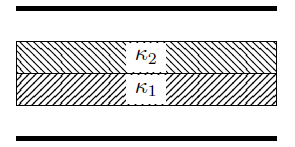
\includegraphics[width=0.5\textwidth]{MixedDielectrics.png}
	\end{center}
\end{figure}

(\textit{Source: modified from Vetri and Dan})

\section{Electric Currents and Resistance}

\subsection{Non-Uniform Resistor}

A resistor is made from two concentric spheres with radii $a$ and $b$ between which there is a material with resistivity that varies with radius as $\rho(r) = \rho_0 \left( \frac{r}{a} \right)^s$, where $\rho_0$ constant. A battery with voltage $V$ is hooked up to the resistor such that current is injected into the resistor from the inner sphere, and removed from the outer sphere.
\begin{enumerate}
	\item If the electric field between the spheres is constant, what is $s$?
	\item What is the current $I$ in the circuit?
\end{enumerate}

(\textit{Source: Vetri and Dan})

\subsection{Making Resistance Constant}

For some applications it is important that the value of resistance does not change. For example, suppose you want to make a resistor of resistance $R$ and you have available two wires with resistivity $\rho_1$ and $\rho_2$ at $T_0=0 ^o C$, both with cross sectional area $A$. We want to make a resistor by combining segments of these two wires. Find the length $l_2$ of the second wire if the first is $l_1$ so that the net resistance is independent of temperature. Suppose that they have fractional changes in resistance of $\alpha_1> 0$, $\alpha_2 < 0$. Also suppose the lengths and areas of the wires does not change with temperatures. (Combine them in series.)
 
(\textit{Source: modified from Giancolli 25-26})

\subsection{Radially Outwards Current and Resistance}

A hollow cylindrical resistor with inner radius $r_1$ and outer radius $r_2$, and length $l$, is made of a material whose resistivity is $\rho$. Show that the resistance is given by $R=\frac{\rho}{2\pi l}ln\frac{r_2}{r_1}$ for current that flows radially outwards.

(\textit{Source: Giancoli 25-30, part (a)})

\subsection{Flashlights}

An ordinary flashlight uses two D-cell 1.5-V batteries connected in series. The bulb draws 380 mA when turned on. (a) Calculate the resistance of the bulb and the power dissipated. (b) By what factor would the power increase if four D-cells in series were used with the same bulb? (Neglect heating effects of the filament.) Why shouldn't you try this?

(\textit{Source: Giancoli 25-42})

\end{document}
